\documentclass[12pt]{article}
\usepackage{mathptmx}
\usepackage[T1]{fontenc}
\usepackage[utf8]{inputenc}
\usepackage[pdftex]{graphicx}
\usepackage{natbib}
\usepackage{hyperref}
\usepackage[left=40mm,right=25mm,bottom=25mm,top=25mm]{geometry}
\usepackage{setspace}
\usepackage{ragged2e}
\usepackage{titlesec}
\usepackage{sectsty}
\usepackage{amsmath}
\usepackage{amsfonts}
\usepackage{amsthm}
\usepackage{amssymb}
\usepackage{mathrsfs}
\usepackage{newtxtext,newtxmath}
\usepackage{indentfirst}
\sectionfont{\fontsize{12}{15}\selectfont}
\subsectionfont{\fontsize{12}{15}\selectfont} 
\subsubsectionfont{\fontsize{12}{15}\selectfont}
\renewcommand{\theequation}{\arabic{section}.\arabic{equation}}
\renewcommand{\thefigure}{\arabic{section}.\arabic{figure}}

\usepackage{adjustbox}
\usepackage{braket}
\usepackage{tabularx}


\begin{document}
\begin{titlepage}
\newgeometry{left=25mm,right=25mm,bottom=25mm,top=25mm}
\begin{center}
\vspace*{1.5cm}\LARGE\textbf{\underline{ISTANBUL TECHNICAL UNIVERSITY}}\vspace*{0.6cm}
\Large\textbf{\underline{FACULTY OF SCIENCE AND LETTERS}}\vspace*{0.6cm}\\
\Large\textbf{Physics Engineering Design I}\vspace*{0.8cm}


\includegraphics[width=0.4\textwidth]{itu-istanbul-teknik_universitesi-logo.png}

\vspace{0.5cm}
\Large\textbf{Title}\vspace{0.5cm}

\large\textbf{Ahmet Ünal}\vspace{0.8cm}

\small\textbf{}

\end{center}
\begin{flushleft}
\textbf{\textit{Department \hspace*{1.7mm}: Physics Engineering}}\\ \vspace{0.4cm}
\textbf{ID \hspace{1.8cm}: 090160503}\\ \vspace{0.4cm}
\textbf{Advisors \hspace{0.85cm}: Doç. Dr. A. Levent Subaşı} \vspace{0.5cm}

\end{flushleft}



\end{titlepage}
%-------------------------------------------------



%---------------------------------------

\onehalfspacing

\pagenumbering{roman}

%---------------------------------------

\section*{\centering{ABSTRACT}}
\justifying

 
\addcontentsline{toc}{section}{ABSTRACT}
\clearpage


%---------------------------------------

\section*{\centering{ACKNOWLEDGEMENTS}}
\justifying 


\addcontentsline{toc}{section}{ACKNOWLEDGEMENTS}
\clearpage

%---------------------------------------

\renewcommand\contentsname{CONTENTS} 
\begingroup
    \let\clearpage\relax
    \tableofcontents
\endgroup
\addcontentsline{toc}{section}{CONTENTS}
\clearpage

%---------------------------------------

\pagenumbering{arabic}

%---------------------------------------

\onehalfspacing

\section{Introduction}
This document is a template for ITU Physics Engineering bachelors graduation project. Refer a figure Fig.~\ref{fig:fig1}, refer a table with Tab.~\ref{tab:tab1}, refer a equation Eq.~\ref{eq:eq1}, cite a document~\cite{sakurai_modern_2010}, cite multiple documents~\cite{sakurai_modern_2010,kramer_quantumopticsjl_2018,baumgratz_quantifying_2014,verstraete_matrix_2008}, refer a section Sec.~\ref{sec:sec1}.



\section{First Section,\label{sec:sec1}}

\subsection{Equation and Table Example}
One line equation with numbering:
\begin{equation}
    H\ket{\Psi}=E\ket{\Psi}
    \label{eq:eq1}
\end{equation}

Multiple line equation:
\begin{equation}\label{eq:pareto mle2}
    \begin{aligned}
        \pmb{\rho}(\theta,\phi)&= \ket{\psi(\theta,\phi)}\bra{\psi(\theta,\phi))}
                  \\ & =\frac{1}{2}\pmb{I}+
        \begin{pmatrix}
               cos(\theta) & sin(\theta/2)e^{-i\phi}\\
               sin(\theta/2)e^{i\phi} & -cos(\theta)
        \end{pmatrix}
                  \\ & =\frac{1}{2}(\pmb{I}+\hat{n}\cdot\vec{\pmb{\sigma}})
    \end{aligned}
\end{equation} 

Table example:

\begin{table}[h!]
  \caption{Example Table}
  \centering
  \label{tab:tab1}
  \begin{tabularx}{\textwidth}{XX}
    \hline\hline
    Spin & Eigenvalue \\
    \hline\hline 
      $\frac{1}{2}$& $\frac{\hslash}{2}$\\
    \hline
    $-\frac{1}{2}$& $-\frac{\hslash}{2}$\\
    \hline
  \end{tabularx}
\end{table}


\subsection{Figure Example}


\begin{figure}[h!]
\centering
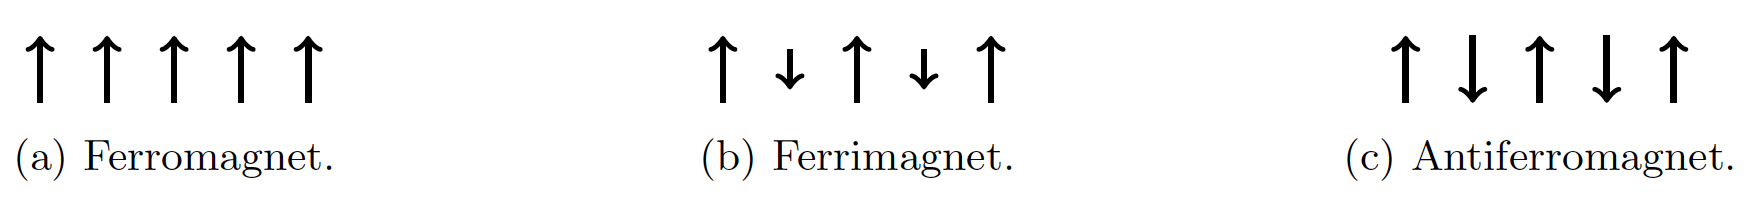
\includegraphics[width=0.6\textwidth]{Pics/Diff Type of Magnets.png}
\caption{Different Types of Magnets}
\label{fig:fig1}
\end{figure}   








 
%-----------------------------------------

\section{Second Section}




\section{Conclusions, Discussions and Future Work}

%-------------------------------------------



\bibliographystyle{unsrt}
\bibliography{mybib}
\addcontentsline{toc}{section}{References}




\end{document}